\documentclass[twoside]{book}

% Packages required by doxygen
\usepackage{fixltx2e}
\usepackage{calc}
\usepackage{doxygen}
\usepackage[export]{adjustbox} % also loads graphicx
\usepackage{graphicx}
\usepackage[utf8]{inputenc}
\usepackage{makeidx}
\usepackage{multicol}
\usepackage{multirow}
\PassOptionsToPackage{warn}{textcomp}
\usepackage{textcomp}
\usepackage[nointegrals]{wasysym}
\usepackage[table]{xcolor}

% Font selection
\usepackage[T1]{fontenc}
\usepackage[scaled=.90]{helvet}
\usepackage{courier}
\usepackage{amssymb}
\usepackage{sectsty}
\renewcommand{\familydefault}{\sfdefault}
\allsectionsfont{%
  \fontseries{bc}\selectfont%
  \color{darkgray}%
}
\renewcommand{\DoxyLabelFont}{%
  \fontseries{bc}\selectfont%
  \color{darkgray}%
}
\newcommand{\+}{\discretionary{\mbox{\scriptsize$\hookleftarrow$}}{}{}}

% Page & text layout
\usepackage{geometry}
\geometry{%
  a4paper,%
  top=2.5cm,%
  bottom=2.5cm,%
  left=2.5cm,%
  right=2.5cm%
}
\tolerance=750
\hfuzz=15pt
\hbadness=750
\setlength{\emergencystretch}{15pt}
\setlength{\parindent}{0cm}
\setlength{\parskip}{3ex plus 2ex minus 2ex}
\makeatletter
\renewcommand{\paragraph}{%
  \@startsection{paragraph}{4}{0ex}{-1.0ex}{1.0ex}{%
    \normalfont\normalsize\bfseries\SS@parafont%
  }%
}
\renewcommand{\subparagraph}{%
  \@startsection{subparagraph}{5}{0ex}{-1.0ex}{1.0ex}{%
    \normalfont\normalsize\bfseries\SS@subparafont%
  }%
}
\makeatother

% Headers & footers
\usepackage{fancyhdr}
\pagestyle{fancyplain}
\fancyhead[LE]{\fancyplain{}{\bfseries\thepage}}
\fancyhead[CE]{\fancyplain{}{}}
\fancyhead[RE]{\fancyplain{}{\bfseries\leftmark}}
\fancyhead[LO]{\fancyplain{}{\bfseries\rightmark}}
\fancyhead[CO]{\fancyplain{}{}}
\fancyhead[RO]{\fancyplain{}{\bfseries\thepage}}
\fancyfoot[LE]{\fancyplain{}{}}
\fancyfoot[CE]{\fancyplain{}{}}
\fancyfoot[RE]{\fancyplain{}{\bfseries\scriptsize Generated by Doxygen }}
\fancyfoot[LO]{\fancyplain{}{\bfseries\scriptsize Generated by Doxygen }}
\fancyfoot[CO]{\fancyplain{}{}}
\fancyfoot[RO]{\fancyplain{}{}}
\renewcommand{\footrulewidth}{0.4pt}
\renewcommand{\chaptermark}[1]{%
  \markboth{#1}{}%
}
\renewcommand{\sectionmark}[1]{%
  \markright{\thesection\ #1}%
}

% Indices & bibliography
\usepackage{natbib}
\usepackage[titles]{tocloft}
\setcounter{tocdepth}{3}
\setcounter{secnumdepth}{5}
\makeindex

% Hyperlinks (required, but should be loaded last)
\usepackage{ifpdf}
\ifpdf
  \usepackage[pdftex,pagebackref=true]{hyperref}
\else
  \usepackage[ps2pdf,pagebackref=true]{hyperref}
\fi
\hypersetup{%
  colorlinks=true,%
  linkcolor=blue,%
  citecolor=blue,%
  unicode%
}

% Custom commands
\newcommand{\clearemptydoublepage}{%
  \newpage{\pagestyle{empty}\cleardoublepage}%
}

\usepackage{caption}
\captionsetup{labelsep=space,justification=centering,font={bf},singlelinecheck=off,skip=4pt,position=top}

%===== C O N T E N T S =====

\begin{document}

% Titlepage & ToC
\hypersetup{pageanchor=false,
             bookmarksnumbered=true,
             pdfencoding=unicode
            }
\pagenumbering{alph}
\begin{titlepage}
\vspace*{7cm}
\begin{center}%
{\Large Open Ephys }\\
\vspace*{1cm}
{\large Generated by Doxygen 1.8.14}\\
\end{center}
\end{titlepage}
\clearemptydoublepage
\pagenumbering{roman}
\tableofcontents
\clearemptydoublepage
\pagenumbering{arabic}
\hypersetup{pageanchor=true}

%--- Begin generated contents ---
\chapter{Welcome to the Open Ephys G\+U\+I!}
\label{index}\hypertarget{index}{}\hypertarget{index_intro}{}\section{Introduction}\label{index_intro}
This is the introduction.\hypertarget{index_install}{}\section{More info}\label{index_install}
\hypertarget{index_step1}{}\subsection{More info will appear here eventually!}\label{index_step1}

\chapter{Namespace Index}
\section{Namespace List}
Here is a list of all namespaces with brief descriptions\+:\begin{DoxyCompactList}
\item\contentsline{section}{\mbox{\hyperlink{namespace_access_class}{Access\+Class}} }{\pageref{namespace_access_class}}{}
\item\contentsline{section}{\mbox{\hyperlink{namespace_core_services}{Core\+Services}} }{\pageref{namespace_core_services}}{}
\item\contentsline{section}{\mbox{\hyperlink{namespace_core_services_1_1_record_node}{Core\+Services\+::\+Record\+Node}} }{\pageref{namespace_core_services_1_1_record_node}}{}
\end{DoxyCompactList}

\chapter{Hierarchical Index}
\section{Class Hierarchy}
This inheritance list is sorted roughly, but not completely, alphabetically\+:\begin{DoxyCompactList}
\item Document\+Window\begin{DoxyCompactList}
\item \contentsline{section}{Main\+Window}{\pageref{class_main_window}}{}
\end{DoxyCompactList}
\item \contentsline{section}{Access\+Class\+:\+:External\+Processor\+Accessor}{\pageref{class_access_class_1_1_external_processor_accessor}}{}
\item J\+U\+C\+E\+Application\begin{DoxyCompactList}
\item \contentsline{section}{Open\+Ephys\+Application}{\pageref{class_open_ephys_application}}{}
\end{DoxyCompactList}
\end{DoxyCompactList}

\chapter{Class Index}
\section{Class List}
Here are the classes, structs, unions and interfaces with brief descriptions\+:\begin{DoxyCompactList}
\item\contentsline{section}{\mbox{\hyperlink{class_access_class_1_1_external_processor_accessor}{Access\+Class\+::\+External\+Processor\+Accessor}} }{\pageref{class_access_class_1_1_external_processor_accessor}}{}
\item\contentsline{section}{\mbox{\hyperlink{class_main_window}{Main\+Window}} }{\pageref{class_main_window}}{}
\item\contentsline{section}{\mbox{\hyperlink{class_open_ephys_application}{Open\+Ephys\+Application}} }{\pageref{class_open_ephys_application}}{}
\end{DoxyCompactList}

\chapter{File Index}
\section{File List}
Here is a list of all files with brief descriptions\+:\begin{DoxyCompactList}
\item\contentsline{section}{Source/\mbox{\hyperlink{_access_class_8cpp}{Access\+Class.\+cpp}} }{\pageref{_access_class_8cpp}}{}
\item\contentsline{section}{Source/\mbox{\hyperlink{_access_class_8h}{Access\+Class.\+h}} }{\pageref{_access_class_8h}}{}
\item\contentsline{section}{Source/\mbox{\hyperlink{_core_services_8cpp}{Core\+Services.\+cpp}} }{\pageref{_core_services_8cpp}}{}
\item\contentsline{section}{Source/\mbox{\hyperlink{_core_services_8h}{Core\+Services.\+h}} }{\pageref{_core_services_8h}}{}
\item\contentsline{section}{Source/\mbox{\hyperlink{_doxygen_main_page_8h}{Doxygen\+Main\+Page.\+h}} }{\pageref{_doxygen_main_page_8h}}{}
\item\contentsline{section}{Source/\mbox{\hyperlink{_main_8cpp}{Main.\+cpp}} }{\pageref{_main_8cpp}}{}
\item\contentsline{section}{Source/\mbox{\hyperlink{_main_window_8cpp}{Main\+Window.\+cpp}} }{\pageref{_main_window_8cpp}}{}
\item\contentsline{section}{Source/\mbox{\hyperlink{_main_window_8h}{Main\+Window.\+h}} }{\pageref{_main_window_8h}}{}
\end{DoxyCompactList}

\chapter{Namespace Documentation}
\hypertarget{namespace_access_class}{}\section{Access\+Class Namespace Reference}
\label{namespace_access_class}\index{Access\+Class@{Access\+Class}}
\subsection*{Classes}
\begin{DoxyCompactItemize}
\item 
class \mbox{\hyperlink{class_access_class_1_1_external_processor_accessor}{External\+Processor\+Accessor}}
\end{DoxyCompactItemize}
\subsection*{Functions}
\begin{DoxyCompactItemize}
\item 
void \mbox{\hyperlink{namespace_access_class_a4f1f8ce54b0d1e3d6319efe95c858e1b}{set\+U\+I\+Component}} (U\+I\+Component $\ast$ui\+\_\+)
\item 
void \mbox{\hyperlink{namespace_access_class_a7a20009ac4b41582f1379b6196f2c07c}{shutdown\+Broadcaster}} ()
\item 
Editor\+Viewport $\ast$ \mbox{\hyperlink{namespace_access_class_a53ff876e8fae76efe1766a3c6b5defc8}{get\+Editor\+Viewport}} ()
\item 
Data\+Viewport $\ast$ \mbox{\hyperlink{namespace_access_class_af26919b327fd17cb4a3ed79623f8795f}{get\+Data\+Viewport}} ()
\item 
Processor\+List $\ast$ \mbox{\hyperlink{namespace_access_class_af8981a34e6624add46145d2a3226c6c7}{get\+Processor\+List}} ()
\item 
Processor\+Graph $\ast$ \mbox{\hyperlink{namespace_access_class_ac50c3de3d49e5d88efb0bdef178523e7}{get\+Processor\+Graph}} ()
\item 
Control\+Panel $\ast$ \mbox{\hyperlink{namespace_access_class_a85b3fce72926c6c93cede477ed7f0dc1}{get\+Control\+Panel}} ()
\item 
Message\+Center\+Editor $\ast$ \mbox{\hyperlink{namespace_access_class_a32785f88b52c58ae0cd1fee7857c1730}{get\+Message\+Center}} ()
\item 
U\+I\+Component $\ast$ \mbox{\hyperlink{namespace_access_class_a847041f47180bab4dd27e7b379f71ce9}{get\+U\+I\+Component}} ()
\item 
Audio\+Component $\ast$ \mbox{\hyperlink{namespace_access_class_a6008b5597fd52fabd69ff28725717287}{get\+Audio\+Component}} ()
\item 
Graph\+Viewer $\ast$ \mbox{\hyperlink{namespace_access_class_a45a325e053c7e866aab251efa1d91008}{get\+Graph\+Viewer}} ()
\item 
Plugin\+Manager $\ast$ \mbox{\hyperlink{namespace_access_class_a23556c0c2fb931081168be89726b7419}{get\+Plugin\+Manager}} ()
\item 
Action\+Broadcaster $\ast$ \mbox{\hyperlink{namespace_access_class_abbdfc97a1cc576d5808d6c9958fdd84f}{get\+Broadcaster}} ()
\end{DoxyCompactItemize}


\subsection{Function Documentation}
\mbox{\Hypertarget{namespace_access_class_a6008b5597fd52fabd69ff28725717287}\label{namespace_access_class_a6008b5597fd52fabd69ff28725717287}} 
\index{Access\+Class@{Access\+Class}!get\+Audio\+Component@{get\+Audio\+Component}}
\index{get\+Audio\+Component@{get\+Audio\+Component}!Access\+Class@{Access\+Class}}
\subsubsection{\texorpdfstring{get\+Audio\+Component()}{getAudioComponent()}}
{\footnotesize\ttfamily Audio\+Component $\ast$ Access\+Class\+::get\+Audio\+Component (\begin{DoxyParamCaption}{ }\end{DoxyParamCaption})}

Returns a pointer to the application\textquotesingle{}s Audio\+Component. \mbox{\Hypertarget{namespace_access_class_abbdfc97a1cc576d5808d6c9958fdd84f}\label{namespace_access_class_abbdfc97a1cc576d5808d6c9958fdd84f}} 
\index{Access\+Class@{Access\+Class}!get\+Broadcaster@{get\+Broadcaster}}
\index{get\+Broadcaster@{get\+Broadcaster}!Access\+Class@{Access\+Class}}
\subsubsection{\texorpdfstring{get\+Broadcaster()}{getBroadcaster()}}
{\footnotesize\ttfamily Action\+Broadcaster $\ast$ Access\+Class\+::get\+Broadcaster (\begin{DoxyParamCaption}{ }\end{DoxyParamCaption})}

\mbox{\Hypertarget{namespace_access_class_a85b3fce72926c6c93cede477ed7f0dc1}\label{namespace_access_class_a85b3fce72926c6c93cede477ed7f0dc1}} 
\index{Access\+Class@{Access\+Class}!get\+Control\+Panel@{get\+Control\+Panel}}
\index{get\+Control\+Panel@{get\+Control\+Panel}!Access\+Class@{Access\+Class}}
\subsubsection{\texorpdfstring{get\+Control\+Panel()}{getControlPanel()}}
{\footnotesize\ttfamily Control\+Panel $\ast$ Access\+Class\+::get\+Control\+Panel (\begin{DoxyParamCaption}{ }\end{DoxyParamCaption})}

Returns a pointer to the application\textquotesingle{}s Data\+Viewport. \mbox{\Hypertarget{namespace_access_class_af26919b327fd17cb4a3ed79623f8795f}\label{namespace_access_class_af26919b327fd17cb4a3ed79623f8795f}} 
\index{Access\+Class@{Access\+Class}!get\+Data\+Viewport@{get\+Data\+Viewport}}
\index{get\+Data\+Viewport@{get\+Data\+Viewport}!Access\+Class@{Access\+Class}}
\subsubsection{\texorpdfstring{get\+Data\+Viewport()}{getDataViewport()}}
{\footnotesize\ttfamily Data\+Viewport $\ast$ Access\+Class\+::get\+Data\+Viewport (\begin{DoxyParamCaption}{ }\end{DoxyParamCaption})}

Returns a pointer to the application\textquotesingle{}s Data\+Viewport. \mbox{\Hypertarget{namespace_access_class_a53ff876e8fae76efe1766a3c6b5defc8}\label{namespace_access_class_a53ff876e8fae76efe1766a3c6b5defc8}} 
\index{Access\+Class@{Access\+Class}!get\+Editor\+Viewport@{get\+Editor\+Viewport}}
\index{get\+Editor\+Viewport@{get\+Editor\+Viewport}!Access\+Class@{Access\+Class}}
\subsubsection{\texorpdfstring{get\+Editor\+Viewport()}{getEditorViewport()}}
{\footnotesize\ttfamily Editor\+Viewport $\ast$ Access\+Class\+::get\+Editor\+Viewport (\begin{DoxyParamCaption}{ }\end{DoxyParamCaption})}

Returns a pointer to the application\textquotesingle{}s Editor\+Viewport. \mbox{\Hypertarget{namespace_access_class_a45a325e053c7e866aab251efa1d91008}\label{namespace_access_class_a45a325e053c7e866aab251efa1d91008}} 
\index{Access\+Class@{Access\+Class}!get\+Graph\+Viewer@{get\+Graph\+Viewer}}
\index{get\+Graph\+Viewer@{get\+Graph\+Viewer}!Access\+Class@{Access\+Class}}
\subsubsection{\texorpdfstring{get\+Graph\+Viewer()}{getGraphViewer()}}
{\footnotesize\ttfamily Graph\+Viewer $\ast$ Access\+Class\+::get\+Graph\+Viewer (\begin{DoxyParamCaption}{ }\end{DoxyParamCaption})}

Returns a pointer to the application\textquotesingle{}s Graph\+Viewer. \mbox{\Hypertarget{namespace_access_class_a32785f88b52c58ae0cd1fee7857c1730}\label{namespace_access_class_a32785f88b52c58ae0cd1fee7857c1730}} 
\index{Access\+Class@{Access\+Class}!get\+Message\+Center@{get\+Message\+Center}}
\index{get\+Message\+Center@{get\+Message\+Center}!Access\+Class@{Access\+Class}}
\subsubsection{\texorpdfstring{get\+Message\+Center()}{getMessageCenter()}}
{\footnotesize\ttfamily Message\+Center\+Editor $\ast$ Access\+Class\+::get\+Message\+Center (\begin{DoxyParamCaption}{ }\end{DoxyParamCaption})}

Returns a pointer to the application\textquotesingle{}s Message\+Center. \mbox{\Hypertarget{namespace_access_class_a23556c0c2fb931081168be89726b7419}\label{namespace_access_class_a23556c0c2fb931081168be89726b7419}} 
\index{Access\+Class@{Access\+Class}!get\+Plugin\+Manager@{get\+Plugin\+Manager}}
\index{get\+Plugin\+Manager@{get\+Plugin\+Manager}!Access\+Class@{Access\+Class}}
\subsubsection{\texorpdfstring{get\+Plugin\+Manager()}{getPluginManager()}}
{\footnotesize\ttfamily Plugin\+Manager $\ast$ Access\+Class\+::get\+Plugin\+Manager (\begin{DoxyParamCaption}{ }\end{DoxyParamCaption})}

Returns a pointer to the application\textquotesingle{}s Plugin\+Manager. \mbox{\Hypertarget{namespace_access_class_ac50c3de3d49e5d88efb0bdef178523e7}\label{namespace_access_class_ac50c3de3d49e5d88efb0bdef178523e7}} 
\index{Access\+Class@{Access\+Class}!get\+Processor\+Graph@{get\+Processor\+Graph}}
\index{get\+Processor\+Graph@{get\+Processor\+Graph}!Access\+Class@{Access\+Class}}
\subsubsection{\texorpdfstring{get\+Processor\+Graph()}{getProcessorGraph()}}
{\footnotesize\ttfamily Processor\+Graph $\ast$ Access\+Class\+::get\+Processor\+Graph (\begin{DoxyParamCaption}{ }\end{DoxyParamCaption})}

Returns a pointer to the application\textquotesingle{}s Processor\+Graph. \mbox{\Hypertarget{namespace_access_class_af8981a34e6624add46145d2a3226c6c7}\label{namespace_access_class_af8981a34e6624add46145d2a3226c6c7}} 
\index{Access\+Class@{Access\+Class}!get\+Processor\+List@{get\+Processor\+List}}
\index{get\+Processor\+List@{get\+Processor\+List}!Access\+Class@{Access\+Class}}
\subsubsection{\texorpdfstring{get\+Processor\+List()}{getProcessorList()}}
{\footnotesize\ttfamily Processor\+List $\ast$ Access\+Class\+::get\+Processor\+List (\begin{DoxyParamCaption}{ }\end{DoxyParamCaption})}

Returns a pointer to the application\textquotesingle{}s Processor\+List. \mbox{\Hypertarget{namespace_access_class_a847041f47180bab4dd27e7b379f71ce9}\label{namespace_access_class_a847041f47180bab4dd27e7b379f71ce9}} 
\index{Access\+Class@{Access\+Class}!get\+U\+I\+Component@{get\+U\+I\+Component}}
\index{get\+U\+I\+Component@{get\+U\+I\+Component}!Access\+Class@{Access\+Class}}
\subsubsection{\texorpdfstring{get\+U\+I\+Component()}{getUIComponent()}}
{\footnotesize\ttfamily U\+I\+Component $\ast$ Access\+Class\+::get\+U\+I\+Component (\begin{DoxyParamCaption}{ }\end{DoxyParamCaption})}

Returns a pointer to the application\textquotesingle{}s U\+I\+Component. \mbox{\Hypertarget{namespace_access_class_a4f1f8ce54b0d1e3d6319efe95c858e1b}\label{namespace_access_class_a4f1f8ce54b0d1e3d6319efe95c858e1b}} 
\index{Access\+Class@{Access\+Class}!set\+U\+I\+Component@{set\+U\+I\+Component}}
\index{set\+U\+I\+Component@{set\+U\+I\+Component}!Access\+Class@{Access\+Class}}
\subsubsection{\texorpdfstring{set\+U\+I\+Component()}{setUIComponent()}}
{\footnotesize\ttfamily void Access\+Class\+::set\+U\+I\+Component (\begin{DoxyParamCaption}\item[{U\+I\+Component $\ast$}]{ }\end{DoxyParamCaption})}

Sets the object\textquotesingle{}s U\+I\+Component and copies all the necessary pointers from the U\+I\+Component. \mbox{\Hypertarget{namespace_access_class_a7a20009ac4b41582f1379b6196f2c07c}\label{namespace_access_class_a7a20009ac4b41582f1379b6196f2c07c}} 
\index{Access\+Class@{Access\+Class}!shutdown\+Broadcaster@{shutdown\+Broadcaster}}
\index{shutdown\+Broadcaster@{shutdown\+Broadcaster}!Access\+Class@{Access\+Class}}
\subsubsection{\texorpdfstring{shutdown\+Broadcaster()}{shutdownBroadcaster()}}
{\footnotesize\ttfamily void Access\+Class\+::shutdown\+Broadcaster (\begin{DoxyParamCaption}{ }\end{DoxyParamCaption})}


\hypertarget{namespace_core_services}{}\section{Core\+Services Namespace Reference}
\label{namespace_core_services}\index{Core\+Services@{Core\+Services}}
\subsection*{Namespaces}
\begin{DoxyCompactItemize}
\item 
 \mbox{\hyperlink{namespace_core_services_1_1_record_node}{Record\+Node}}
\end{DoxyCompactItemize}
\subsection*{Functions}
\begin{DoxyCompactItemize}
\item 
void \mbox{\hyperlink{namespace_core_services_a2e53c32783c6caa3d66afb7172dc61fd}{update\+Signal\+Chain}} (Generic\+Editor $\ast$source)
\item 
bool \mbox{\hyperlink{namespace_core_services_a877cdc8ef0b6ea0dce61575de663c6f3}{get\+Recording\+Status}} ()
\item 
void \mbox{\hyperlink{namespace_core_services_a70b56adbc7be044f913f088a162a69fd}{set\+Recording\+Status}} (bool enable)
\item 
bool \mbox{\hyperlink{namespace_core_services_afe3e006d8ad41f122bd0d68b9d5976b0}{get\+Acquisition\+Status}} ()
\item 
void \mbox{\hyperlink{namespace_core_services_a93b4f6a705bead14ce6caa04355b03ba}{set\+Acquisition\+Status}} (bool enable)
\item 
void \mbox{\hyperlink{namespace_core_services_a78fdbd1d2b88cc908e60559b47d8a77e}{send\+Status\+Message}} (const String \&text)
\item 
void \mbox{\hyperlink{namespace_core_services_aafd9eeb68c631f37fa234eee4eb8fbca}{send\+Status\+Message}} (const char $\ast$text)
\item 
void \mbox{\hyperlink{namespace_core_services_a3b017a18a0a09b6c4e2fa4af4c5df11e}{highlight\+Editor}} (Generic\+Editor $\ast$ed)
\item 
juce\+::int64 \mbox{\hyperlink{namespace_core_services_a79defb96087c3bddcb388a29a38d6952}{get\+Global\+Timestamp}} ()
\item 
juce\+::int64 \mbox{\hyperlink{namespace_core_services_ad1083e5525ad9ebd19afd9364f122059}{get\+Software\+Timestamp}} ()
\item 
float \mbox{\hyperlink{namespace_core_services_ac9fb78e241aa3805b05d206c78ecfca1}{get\+Global\+Sample\+Rate}} ()
\item 
float \mbox{\hyperlink{namespace_core_services_a1ce836de202979c7c8a8e4f4d42c87f4}{get\+Software\+Sample\+Rate}} ()
\item 
void \mbox{\hyperlink{namespace_core_services_a5b804cf3cba68340baeb3b7c7173b530}{set\+Recording\+Directory}} (String dir)
\item 
void \mbox{\hyperlink{namespace_core_services_a450d2d9574435570b5e4e38caaeb05d7}{create\+New\+Recording\+Dir}} ()
\item 
void \mbox{\hyperlink{namespace_core_services_a2ea8b92387e1ae7ce51180a3861e528c}{set\+Prepend\+Text\+To\+Recording\+Dir}} (String text)
\item 
void \mbox{\hyperlink{namespace_core_services_a75af2d5d3262b95e16bd51fe28a7e26d}{set\+Append\+Text\+To\+Recording\+Dir}} (String text)
\item 
String \mbox{\hyperlink{namespace_core_services_a03eb76579ab53edf169064232a0e2b62}{get\+Selected\+Record\+Engine\+Id}} ()
\item 
bool \mbox{\hyperlink{namespace_core_services_a5c4ad031dbb70b1ca2824a12e65dec86}{set\+Selected\+Record\+Engine\+Id}} (String id)
\item 
const char $\ast$ \mbox{\hyperlink{namespace_core_services_a40705adde6940ed1b94cf880a0cc54a0}{get\+Application\+Resource}} (const char $\ast$name, int \&size)
\item 
File \mbox{\hyperlink{namespace_core_services_a25f9182255aa7c83144c5f65819493bc}{get\+Default\+User\+Save\+Directory}} ()
\item 
String \mbox{\hyperlink{namespace_core_services_a93a10ea82325f2a1baf74ee22e5dbd23}{get\+G\+U\+I\+Version}} ()
\end{DoxyCompactItemize}


\subsection{Function Documentation}
\mbox{\Hypertarget{namespace_core_services_a450d2d9574435570b5e4e38caaeb05d7}\label{namespace_core_services_a450d2d9574435570b5e4e38caaeb05d7}} 
\index{Core\+Services@{Core\+Services}!create\+New\+Recording\+Dir@{create\+New\+Recording\+Dir}}
\index{create\+New\+Recording\+Dir@{create\+New\+Recording\+Dir}!Core\+Services@{Core\+Services}}
\subsubsection{\texorpdfstring{create\+New\+Recording\+Dir()}{createNewRecordingDir()}}
{\footnotesize\ttfamily P\+L\+U\+G\+I\+N\+\_\+\+A\+PI void Core\+Services\+::create\+New\+Recording\+Dir (\begin{DoxyParamCaption}{ }\end{DoxyParamCaption})}

Create new recording directory \mbox{\Hypertarget{namespace_core_services_afe3e006d8ad41f122bd0d68b9d5976b0}\label{namespace_core_services_afe3e006d8ad41f122bd0d68b9d5976b0}} 
\index{Core\+Services@{Core\+Services}!get\+Acquisition\+Status@{get\+Acquisition\+Status}}
\index{get\+Acquisition\+Status@{get\+Acquisition\+Status}!Core\+Services@{Core\+Services}}
\subsubsection{\texorpdfstring{get\+Acquisition\+Status()}{getAcquisitionStatus()}}
{\footnotesize\ttfamily P\+L\+U\+G\+I\+N\+\_\+\+A\+PI bool Core\+Services\+::get\+Acquisition\+Status (\begin{DoxyParamCaption}{ }\end{DoxyParamCaption})}

Returns true if the G\+UI is acquiring data \mbox{\Hypertarget{namespace_core_services_a40705adde6940ed1b94cf880a0cc54a0}\label{namespace_core_services_a40705adde6940ed1b94cf880a0cc54a0}} 
\index{Core\+Services@{Core\+Services}!get\+Application\+Resource@{get\+Application\+Resource}}
\index{get\+Application\+Resource@{get\+Application\+Resource}!Core\+Services@{Core\+Services}}
\subsubsection{\texorpdfstring{get\+Application\+Resource()}{getApplicationResource()}}
{\footnotesize\ttfamily P\+L\+U\+G\+I\+N\+\_\+\+A\+PI const char $\ast$ Core\+Services\+::get\+Application\+Resource (\begin{DoxyParamCaption}\item[{const char $\ast$}]{name,  }\item[{int \&}]{size }\end{DoxyParamCaption})}

\mbox{\Hypertarget{namespace_core_services_a25f9182255aa7c83144c5f65819493bc}\label{namespace_core_services_a25f9182255aa7c83144c5f65819493bc}} 
\index{Core\+Services@{Core\+Services}!get\+Default\+User\+Save\+Directory@{get\+Default\+User\+Save\+Directory}}
\index{get\+Default\+User\+Save\+Directory@{get\+Default\+User\+Save\+Directory}!Core\+Services@{Core\+Services}}
\subsubsection{\texorpdfstring{get\+Default\+User\+Save\+Directory()}{getDefaultUserSaveDirectory()}}
{\footnotesize\ttfamily P\+L\+U\+G\+I\+N\+\_\+\+A\+PI File Core\+Services\+::get\+Default\+User\+Save\+Directory (\begin{DoxyParamCaption}{ }\end{DoxyParamCaption})}

Gets the default directory for user-\/initiated file saving/loading \mbox{\Hypertarget{namespace_core_services_ac9fb78e241aa3805b05d206c78ecfca1}\label{namespace_core_services_ac9fb78e241aa3805b05d206c78ecfca1}} 
\index{Core\+Services@{Core\+Services}!get\+Global\+Sample\+Rate@{get\+Global\+Sample\+Rate}}
\index{get\+Global\+Sample\+Rate@{get\+Global\+Sample\+Rate}!Core\+Services@{Core\+Services}}
\subsubsection{\texorpdfstring{get\+Global\+Sample\+Rate()}{getGlobalSampleRate()}}
{\footnotesize\ttfamily P\+L\+U\+G\+I\+N\+\_\+\+A\+PI float Core\+Services\+::get\+Global\+Sample\+Rate (\begin{DoxyParamCaption}{ }\end{DoxyParamCaption})}

Gets the sample rate selected on the Message\+Center interface Defaults to the dample rate of the first hardware source or the software high resolution timer if no hardware source is present \mbox{\Hypertarget{namespace_core_services_a79defb96087c3bddcb388a29a38d6952}\label{namespace_core_services_a79defb96087c3bddcb388a29a38d6952}} 
\index{Core\+Services@{Core\+Services}!get\+Global\+Timestamp@{get\+Global\+Timestamp}}
\index{get\+Global\+Timestamp@{get\+Global\+Timestamp}!Core\+Services@{Core\+Services}}
\subsubsection{\texorpdfstring{get\+Global\+Timestamp()}{getGlobalTimestamp()}}
{\footnotesize\ttfamily P\+L\+U\+G\+I\+N\+\_\+\+A\+PI juce\+::int64 Core\+Services\+::get\+Global\+Timestamp (\begin{DoxyParamCaption}{ }\end{DoxyParamCaption})}

Gets the timestamp selected on the Message\+Center interface Defaults to the first hardware timestamp source or the software one if no hardware timestamping is present \mbox{\Hypertarget{namespace_core_services_a93a10ea82325f2a1baf74ee22e5dbd23}\label{namespace_core_services_a93a10ea82325f2a1baf74ee22e5dbd23}} 
\index{Core\+Services@{Core\+Services}!get\+G\+U\+I\+Version@{get\+G\+U\+I\+Version}}
\index{get\+G\+U\+I\+Version@{get\+G\+U\+I\+Version}!Core\+Services@{Core\+Services}}
\subsubsection{\texorpdfstring{get\+G\+U\+I\+Version()}{getGUIVersion()}}
{\footnotesize\ttfamily P\+L\+U\+G\+I\+N\+\_\+\+A\+PI String Core\+Services\+::get\+G\+U\+I\+Version (\begin{DoxyParamCaption}{ }\end{DoxyParamCaption})}

Gets the G\+UI version \mbox{\Hypertarget{namespace_core_services_a877cdc8ef0b6ea0dce61575de663c6f3}\label{namespace_core_services_a877cdc8ef0b6ea0dce61575de663c6f3}} 
\index{Core\+Services@{Core\+Services}!get\+Recording\+Status@{get\+Recording\+Status}}
\index{get\+Recording\+Status@{get\+Recording\+Status}!Core\+Services@{Core\+Services}}
\subsubsection{\texorpdfstring{get\+Recording\+Status()}{getRecordingStatus()}}
{\footnotesize\ttfamily P\+L\+U\+G\+I\+N\+\_\+\+A\+PI bool Core\+Services\+::get\+Recording\+Status (\begin{DoxyParamCaption}{ }\end{DoxyParamCaption})}

Returns true is the G\+UI is recording \mbox{\Hypertarget{namespace_core_services_a03eb76579ab53edf169064232a0e2b62}\label{namespace_core_services_a03eb76579ab53edf169064232a0e2b62}} 
\index{Core\+Services@{Core\+Services}!get\+Selected\+Record\+Engine\+Id@{get\+Selected\+Record\+Engine\+Id}}
\index{get\+Selected\+Record\+Engine\+Id@{get\+Selected\+Record\+Engine\+Id}!Core\+Services@{Core\+Services}}
\subsubsection{\texorpdfstring{get\+Selected\+Record\+Engine\+Id()}{getSelectedRecordEngineId()}}
{\footnotesize\ttfamily P\+L\+U\+G\+I\+N\+\_\+\+A\+PI String Core\+Services\+::get\+Selected\+Record\+Engine\+Id (\begin{DoxyParamCaption}{ }\end{DoxyParamCaption})}

Gets the ID fo the selected Record Engine \mbox{\Hypertarget{namespace_core_services_a1ce836de202979c7c8a8e4f4d42c87f4}\label{namespace_core_services_a1ce836de202979c7c8a8e4f4d42c87f4}} 
\index{Core\+Services@{Core\+Services}!get\+Software\+Sample\+Rate@{get\+Software\+Sample\+Rate}}
\index{get\+Software\+Sample\+Rate@{get\+Software\+Sample\+Rate}!Core\+Services@{Core\+Services}}
\subsubsection{\texorpdfstring{get\+Software\+Sample\+Rate()}{getSoftwareSampleRate()}}
{\footnotesize\ttfamily P\+L\+U\+G\+I\+N\+\_\+\+A\+PI float Core\+Services\+::get\+Software\+Sample\+Rate (\begin{DoxyParamCaption}{ }\end{DoxyParamCaption})}

Gets the ticker frequency of the software timestamp clock \mbox{\Hypertarget{namespace_core_services_ad1083e5525ad9ebd19afd9364f122059}\label{namespace_core_services_ad1083e5525ad9ebd19afd9364f122059}} 
\index{Core\+Services@{Core\+Services}!get\+Software\+Timestamp@{get\+Software\+Timestamp}}
\index{get\+Software\+Timestamp@{get\+Software\+Timestamp}!Core\+Services@{Core\+Services}}
\subsubsection{\texorpdfstring{get\+Software\+Timestamp()}{getSoftwareTimestamp()}}
{\footnotesize\ttfamily P\+L\+U\+G\+I\+N\+\_\+\+A\+PI juce\+::int64 Core\+Services\+::get\+Software\+Timestamp (\begin{DoxyParamCaption}{ }\end{DoxyParamCaption})}

Gets the software timestamp based on a high resolution timer aligned to the start of each processing block \mbox{\Hypertarget{namespace_core_services_a3b017a18a0a09b6c4e2fa4af4c5df11e}\label{namespace_core_services_a3b017a18a0a09b6c4e2fa4af4c5df11e}} 
\index{Core\+Services@{Core\+Services}!highlight\+Editor@{highlight\+Editor}}
\index{highlight\+Editor@{highlight\+Editor}!Core\+Services@{Core\+Services}}
\subsubsection{\texorpdfstring{highlight\+Editor()}{highlightEditor()}}
{\footnotesize\ttfamily P\+L\+U\+G\+I\+N\+\_\+\+A\+PI void Core\+Services\+::highlight\+Editor (\begin{DoxyParamCaption}\item[{Generic\+Editor $\ast$}]{ed }\end{DoxyParamCaption})}

Highlights an editor \mbox{\Hypertarget{namespace_core_services_a78fdbd1d2b88cc908e60559b47d8a77e}\label{namespace_core_services_a78fdbd1d2b88cc908e60559b47d8a77e}} 
\index{Core\+Services@{Core\+Services}!send\+Status\+Message@{send\+Status\+Message}}
\index{send\+Status\+Message@{send\+Status\+Message}!Core\+Services@{Core\+Services}}
\subsubsection{\texorpdfstring{send\+Status\+Message()}{sendStatusMessage()}\hspace{0.1cm}{\footnotesize\ttfamily [1/2]}}
{\footnotesize\ttfamily P\+L\+U\+G\+I\+N\+\_\+\+A\+PI void Core\+Services\+::send\+Status\+Message (\begin{DoxyParamCaption}\item[{const String \&}]{text }\end{DoxyParamCaption})}

Sends a string to the message bar \mbox{\Hypertarget{namespace_core_services_aafd9eeb68c631f37fa234eee4eb8fbca}\label{namespace_core_services_aafd9eeb68c631f37fa234eee4eb8fbca}} 
\index{Core\+Services@{Core\+Services}!send\+Status\+Message@{send\+Status\+Message}}
\index{send\+Status\+Message@{send\+Status\+Message}!Core\+Services@{Core\+Services}}
\subsubsection{\texorpdfstring{send\+Status\+Message()}{sendStatusMessage()}\hspace{0.1cm}{\footnotesize\ttfamily [2/2]}}
{\footnotesize\ttfamily P\+L\+U\+G\+I\+N\+\_\+\+A\+PI void Core\+Services\+::send\+Status\+Message (\begin{DoxyParamCaption}\item[{const char $\ast$}]{text }\end{DoxyParamCaption})}

Sends a string to the message bar \mbox{\Hypertarget{namespace_core_services_a93b4f6a705bead14ce6caa04355b03ba}\label{namespace_core_services_a93b4f6a705bead14ce6caa04355b03ba}} 
\index{Core\+Services@{Core\+Services}!set\+Acquisition\+Status@{set\+Acquisition\+Status}}
\index{set\+Acquisition\+Status@{set\+Acquisition\+Status}!Core\+Services@{Core\+Services}}
\subsubsection{\texorpdfstring{set\+Acquisition\+Status()}{setAcquisitionStatus()}}
{\footnotesize\ttfamily P\+L\+U\+G\+I\+N\+\_\+\+A\+PI void Core\+Services\+::set\+Acquisition\+Status (\begin{DoxyParamCaption}\item[{bool}]{enable }\end{DoxyParamCaption})}

Activates or deactivates data acquisition \mbox{\Hypertarget{namespace_core_services_a75af2d5d3262b95e16bd51fe28a7e26d}\label{namespace_core_services_a75af2d5d3262b95e16bd51fe28a7e26d}} 
\index{Core\+Services@{Core\+Services}!set\+Append\+Text\+To\+Recording\+Dir@{set\+Append\+Text\+To\+Recording\+Dir}}
\index{set\+Append\+Text\+To\+Recording\+Dir@{set\+Append\+Text\+To\+Recording\+Dir}!Core\+Services@{Core\+Services}}
\subsubsection{\texorpdfstring{set\+Append\+Text\+To\+Recording\+Dir()}{setAppendTextToRecordingDir()}}
{\footnotesize\ttfamily P\+L\+U\+G\+I\+N\+\_\+\+A\+PI void Core\+Services\+::set\+Append\+Text\+To\+Recording\+Dir (\begin{DoxyParamCaption}\item[{String}]{text }\end{DoxyParamCaption})}

Manually set the text to be appended to the recording directory \mbox{\Hypertarget{namespace_core_services_a2ea8b92387e1ae7ce51180a3861e528c}\label{namespace_core_services_a2ea8b92387e1ae7ce51180a3861e528c}} 
\index{Core\+Services@{Core\+Services}!set\+Prepend\+Text\+To\+Recording\+Dir@{set\+Prepend\+Text\+To\+Recording\+Dir}}
\index{set\+Prepend\+Text\+To\+Recording\+Dir@{set\+Prepend\+Text\+To\+Recording\+Dir}!Core\+Services@{Core\+Services}}
\subsubsection{\texorpdfstring{set\+Prepend\+Text\+To\+Recording\+Dir()}{setPrependTextToRecordingDir()}}
{\footnotesize\ttfamily P\+L\+U\+G\+I\+N\+\_\+\+A\+PI void Core\+Services\+::set\+Prepend\+Text\+To\+Recording\+Dir (\begin{DoxyParamCaption}\item[{String}]{text }\end{DoxyParamCaption})}

Manually set the text to be prepended to the recording directory \mbox{\Hypertarget{namespace_core_services_a5b804cf3cba68340baeb3b7c7173b530}\label{namespace_core_services_a5b804cf3cba68340baeb3b7c7173b530}} 
\index{Core\+Services@{Core\+Services}!set\+Recording\+Directory@{set\+Recording\+Directory}}
\index{set\+Recording\+Directory@{set\+Recording\+Directory}!Core\+Services@{Core\+Services}}
\subsubsection{\texorpdfstring{set\+Recording\+Directory()}{setRecordingDirectory()}}
{\footnotesize\ttfamily P\+L\+U\+G\+I\+N\+\_\+\+A\+PI void Core\+Services\+::set\+Recording\+Directory (\begin{DoxyParamCaption}\item[{String}]{dir }\end{DoxyParamCaption})}

Set new recording directory \mbox{\Hypertarget{namespace_core_services_a70b56adbc7be044f913f088a162a69fd}\label{namespace_core_services_a70b56adbc7be044f913f088a162a69fd}} 
\index{Core\+Services@{Core\+Services}!set\+Recording\+Status@{set\+Recording\+Status}}
\index{set\+Recording\+Status@{set\+Recording\+Status}!Core\+Services@{Core\+Services}}
\subsubsection{\texorpdfstring{set\+Recording\+Status()}{setRecordingStatus()}}
{\footnotesize\ttfamily P\+L\+U\+G\+I\+N\+\_\+\+A\+PI void Core\+Services\+::set\+Recording\+Status (\begin{DoxyParamCaption}\item[{bool}]{enable }\end{DoxyParamCaption})}

Activated or deactivates recording \mbox{\Hypertarget{namespace_core_services_a5c4ad031dbb70b1ca2824a12e65dec86}\label{namespace_core_services_a5c4ad031dbb70b1ca2824a12e65dec86}} 
\index{Core\+Services@{Core\+Services}!set\+Selected\+Record\+Engine\+Id@{set\+Selected\+Record\+Engine\+Id}}
\index{set\+Selected\+Record\+Engine\+Id@{set\+Selected\+Record\+Engine\+Id}!Core\+Services@{Core\+Services}}
\subsubsection{\texorpdfstring{set\+Selected\+Record\+Engine\+Id()}{setSelectedRecordEngineId()}}
{\footnotesize\ttfamily P\+L\+U\+G\+I\+N\+\_\+\+A\+PI bool Core\+Services\+::set\+Selected\+Record\+Engine\+Id (\begin{DoxyParamCaption}\item[{String}]{id }\end{DoxyParamCaption})}

Sets a specific Record\+Engine to be used based on its id. Return true if there is an engine with the specified ID and it\textquotesingle{}s possible to change the current engine or false otherwise. \mbox{\Hypertarget{namespace_core_services_a2e53c32783c6caa3d66afb7172dc61fd}\label{namespace_core_services_a2e53c32783c6caa3d66afb7172dc61fd}} 
\index{Core\+Services@{Core\+Services}!update\+Signal\+Chain@{update\+Signal\+Chain}}
\index{update\+Signal\+Chain@{update\+Signal\+Chain}!Core\+Services@{Core\+Services}}
\subsubsection{\texorpdfstring{update\+Signal\+Chain()}{updateSignalChain()}}
{\footnotesize\ttfamily P\+L\+U\+G\+I\+N\+\_\+\+A\+PI void Core\+Services\+::update\+Signal\+Chain (\begin{DoxyParamCaption}\item[{Generic\+Editor $\ast$}]{source }\end{DoxyParamCaption})}

Issues a signal chain update, useful for propagating new channel settings 
\hypertarget{namespace_core_services_1_1_record_node}{}\section{Core\+Services\+:\+:Record\+Node Namespace Reference}
\label{namespace_core_services_1_1_record_node}\index{Core\+Services\+::\+Record\+Node@{Core\+Services\+::\+Record\+Node}}
\subsection*{Functions}
\begin{DoxyCompactItemize}
\item 
void \mbox{\hyperlink{namespace_core_services_1_1_record_node_a5a5d166b16a7990cda9d1667cca88031}{create\+Newrecording\+Dir}} ()
\item 
File \mbox{\hyperlink{namespace_core_services_1_1_record_node_aacbae8c35805cac138be95000a31baa2}{get\+Recording\+Path}} ()
\item 
int \mbox{\hyperlink{namespace_core_services_1_1_record_node_a9652eb6869f905f2b131245f62ddaaf1}{get\+Recording\+Number}} ()
\item 
int \mbox{\hyperlink{namespace_core_services_1_1_record_node_aae47e9fe985ef57735c937bbe8379fa7}{get\+Experiment\+Number}} ()
\item 
void \mbox{\hyperlink{namespace_core_services_1_1_record_node_a9475537f3223762f9e1b852ec8d59811}{write\+Spike}} (const Spike\+Event $\ast$spike, const Spike\+Channel $\ast$chan)
\item 
void \mbox{\hyperlink{namespace_core_services_1_1_record_node_a28b8d2f049b63dc524b27a9ae8bc88fe}{register\+Spike\+Source}} (Generic\+Processor $\ast$processor)
\item 
int \mbox{\hyperlink{namespace_core_services_1_1_record_node_a78a757804cb37410aeb3349594030895}{add\+Spike\+Electrode}} (const Spike\+Channel $\ast$elec)
\end{DoxyCompactItemize}


\subsection{Function Documentation}
\mbox{\Hypertarget{namespace_core_services_1_1_record_node_a78a757804cb37410aeb3349594030895}\label{namespace_core_services_1_1_record_node_a78a757804cb37410aeb3349594030895}} 
\index{Core\+Services\+::\+Record\+Node@{Core\+Services\+::\+Record\+Node}!add\+Spike\+Electrode@{add\+Spike\+Electrode}}
\index{add\+Spike\+Electrode@{add\+Spike\+Electrode}!Core\+Services\+::\+Record\+Node@{Core\+Services\+::\+Record\+Node}}
\subsubsection{\texorpdfstring{add\+Spike\+Electrode()}{addSpikeElectrode()}}
{\footnotesize\ttfamily P\+L\+U\+G\+I\+N\+\_\+\+A\+PI int Core\+Services\+::\+Record\+Node\+::add\+Spike\+Electrode (\begin{DoxyParamCaption}\item[{const Spike\+Channel $\ast$}]{elec }\end{DoxyParamCaption})}

\mbox{\Hypertarget{namespace_core_services_1_1_record_node_a5a5d166b16a7990cda9d1667cca88031}\label{namespace_core_services_1_1_record_node_a5a5d166b16a7990cda9d1667cca88031}} 
\index{Core\+Services\+::\+Record\+Node@{Core\+Services\+::\+Record\+Node}!create\+Newrecording\+Dir@{create\+Newrecording\+Dir}}
\index{create\+Newrecording\+Dir@{create\+Newrecording\+Dir}!Core\+Services\+::\+Record\+Node@{Core\+Services\+::\+Record\+Node}}
\subsubsection{\texorpdfstring{create\+Newrecording\+Dir()}{createNewrecordingDir()}}
{\footnotesize\ttfamily P\+L\+U\+G\+I\+N\+\_\+\+A\+PI void Core\+Services\+::\+Record\+Node\+::create\+Newrecording\+Dir (\begin{DoxyParamCaption}{ }\end{DoxyParamCaption})}

Forces creation of new directory on recording \mbox{\Hypertarget{namespace_core_services_1_1_record_node_aae47e9fe985ef57735c937bbe8379fa7}\label{namespace_core_services_1_1_record_node_aae47e9fe985ef57735c937bbe8379fa7}} 
\index{Core\+Services\+::\+Record\+Node@{Core\+Services\+::\+Record\+Node}!get\+Experiment\+Number@{get\+Experiment\+Number}}
\index{get\+Experiment\+Number@{get\+Experiment\+Number}!Core\+Services\+::\+Record\+Node@{Core\+Services\+::\+Record\+Node}}
\subsubsection{\texorpdfstring{get\+Experiment\+Number()}{getExperimentNumber()}}
{\footnotesize\ttfamily P\+L\+U\+G\+I\+N\+\_\+\+A\+PI int Core\+Services\+::\+Record\+Node\+::get\+Experiment\+Number (\begin{DoxyParamCaption}{ }\end{DoxyParamCaption})}

\mbox{\Hypertarget{namespace_core_services_1_1_record_node_a9652eb6869f905f2b131245f62ddaaf1}\label{namespace_core_services_1_1_record_node_a9652eb6869f905f2b131245f62ddaaf1}} 
\index{Core\+Services\+::\+Record\+Node@{Core\+Services\+::\+Record\+Node}!get\+Recording\+Number@{get\+Recording\+Number}}
\index{get\+Recording\+Number@{get\+Recording\+Number}!Core\+Services\+::\+Record\+Node@{Core\+Services\+::\+Record\+Node}}
\subsubsection{\texorpdfstring{get\+Recording\+Number()}{getRecordingNumber()}}
{\footnotesize\ttfamily P\+L\+U\+G\+I\+N\+\_\+\+A\+PI int Core\+Services\+::\+Record\+Node\+::get\+Recording\+Number (\begin{DoxyParamCaption}{ }\end{DoxyParamCaption})}

\mbox{\Hypertarget{namespace_core_services_1_1_record_node_aacbae8c35805cac138be95000a31baa2}\label{namespace_core_services_1_1_record_node_aacbae8c35805cac138be95000a31baa2}} 
\index{Core\+Services\+::\+Record\+Node@{Core\+Services\+::\+Record\+Node}!get\+Recording\+Path@{get\+Recording\+Path}}
\index{get\+Recording\+Path@{get\+Recording\+Path}!Core\+Services\+::\+Record\+Node@{Core\+Services\+::\+Record\+Node}}
\subsubsection{\texorpdfstring{get\+Recording\+Path()}{getRecordingPath()}}
{\footnotesize\ttfamily P\+L\+U\+G\+I\+N\+\_\+\+A\+PI File Core\+Services\+::\+Record\+Node\+::get\+Recording\+Path (\begin{DoxyParamCaption}{ }\end{DoxyParamCaption})}

Gets the current recording directories and status information \mbox{\Hypertarget{namespace_core_services_1_1_record_node_a28b8d2f049b63dc524b27a9ae8bc88fe}\label{namespace_core_services_1_1_record_node_a28b8d2f049b63dc524b27a9ae8bc88fe}} 
\index{Core\+Services\+::\+Record\+Node@{Core\+Services\+::\+Record\+Node}!register\+Spike\+Source@{register\+Spike\+Source}}
\index{register\+Spike\+Source@{register\+Spike\+Source}!Core\+Services\+::\+Record\+Node@{Core\+Services\+::\+Record\+Node}}
\subsubsection{\texorpdfstring{register\+Spike\+Source()}{registerSpikeSource()}}
{\footnotesize\ttfamily P\+L\+U\+G\+I\+N\+\_\+\+A\+PI void Core\+Services\+::\+Record\+Node\+::register\+Spike\+Source (\begin{DoxyParamCaption}\item[{Generic\+Processor $\ast$}]{processor }\end{DoxyParamCaption})}

\mbox{\Hypertarget{namespace_core_services_1_1_record_node_a9475537f3223762f9e1b852ec8d59811}\label{namespace_core_services_1_1_record_node_a9475537f3223762f9e1b852ec8d59811}} 
\index{Core\+Services\+::\+Record\+Node@{Core\+Services\+::\+Record\+Node}!write\+Spike@{write\+Spike}}
\index{write\+Spike@{write\+Spike}!Core\+Services\+::\+Record\+Node@{Core\+Services\+::\+Record\+Node}}
\subsubsection{\texorpdfstring{write\+Spike()}{writeSpike()}}
{\footnotesize\ttfamily P\+L\+U\+G\+I\+N\+\_\+\+A\+PI void Core\+Services\+::\+Record\+Node\+::write\+Spike (\begin{DoxyParamCaption}\item[{const Spike\+Event $\ast$}]{spike,  }\item[{const Spike\+Channel $\ast$}]{chan }\end{DoxyParamCaption})}


\chapter{Class Documentation}
\hypertarget{class_access_class_1_1_external_processor_accessor}{}\section{Access\+Class\+:\+:External\+Processor\+Accessor Class Reference}
\label{class_access_class_1_1_external_processor_accessor}\index{Access\+Class\+::\+External\+Processor\+Accessor@{Access\+Class\+::\+External\+Processor\+Accessor}}


{\ttfamily \#include $<$Access\+Class.\+h$>$}

\subsection*{Static Public Member Functions}
\begin{DoxyCompactItemize}
\item 
static Midi\+Buffer $\ast$ \mbox{\hyperlink{class_access_class_1_1_external_processor_accessor_a698423b149b9ff58758920993efb0936}{get\+Midi\+Buffer}} (Generic\+Processor $\ast$proc)
\end{DoxyCompactItemize}


\subsection{Member Function Documentation}
\mbox{\Hypertarget{class_access_class_1_1_external_processor_accessor_a698423b149b9ff58758920993efb0936}\label{class_access_class_1_1_external_processor_accessor_a698423b149b9ff58758920993efb0936}} 
\index{Access\+Class\+::\+External\+Processor\+Accessor@{Access\+Class\+::\+External\+Processor\+Accessor}!get\+Midi\+Buffer@{get\+Midi\+Buffer}}
\index{get\+Midi\+Buffer@{get\+Midi\+Buffer}!Access\+Class\+::\+External\+Processor\+Accessor@{Access\+Class\+::\+External\+Processor\+Accessor}}
\subsubsection{\texorpdfstring{get\+Midi\+Buffer()}{getMidiBuffer()}}
{\footnotesize\ttfamily Midi\+Buffer $\ast$ Access\+Class\+::\+External\+Processor\+Accessor\+::get\+Midi\+Buffer (\begin{DoxyParamCaption}\item[{Generic\+Processor $\ast$}]{proc }\end{DoxyParamCaption})\hspace{0.3cm}{\ttfamily [static]}}



The documentation for this class was generated from the following files\+:\begin{DoxyCompactItemize}
\item 
Source/\mbox{\hyperlink{_access_class_8h}{Access\+Class.\+h}}\item 
Source/\mbox{\hyperlink{_access_class_8cpp}{Access\+Class.\+cpp}}\end{DoxyCompactItemize}

\hypertarget{class_main_window}{}\section{Main\+Window Class Reference}
\label{class_main_window}\index{Main\+Window@{Main\+Window}}


{\ttfamily \#include $<$Main\+Window.\+h$>$}

Inheritance diagram for Main\+Window\+:\begin{figure}[H]
\begin{center}
\leavevmode
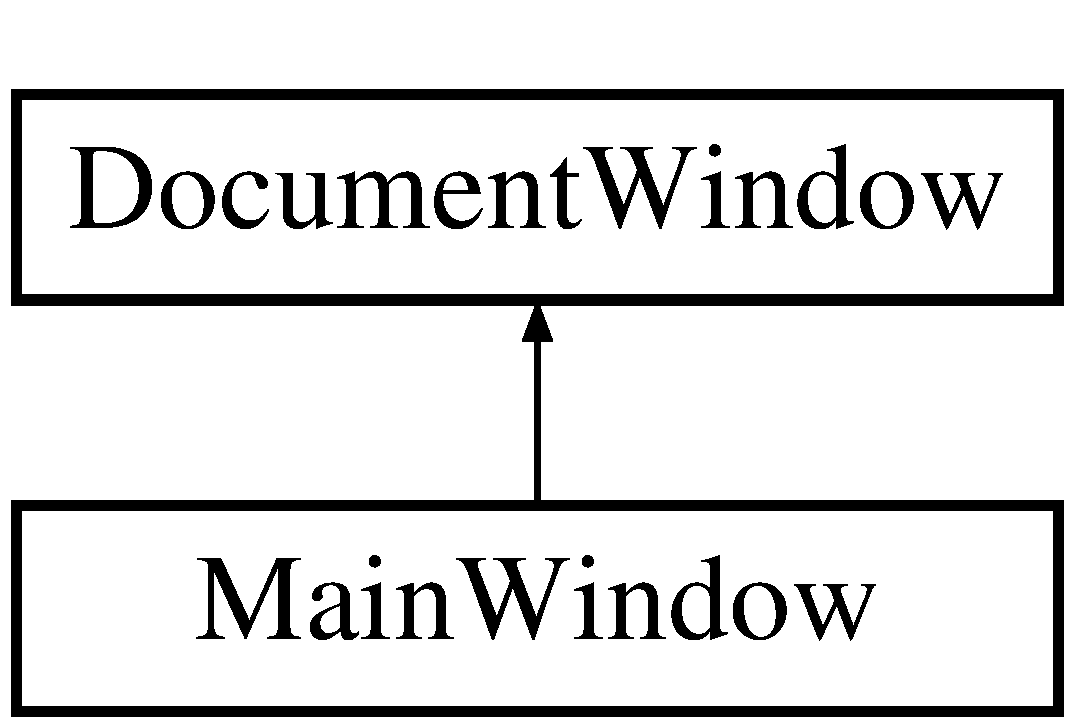
\includegraphics[height=2.000000cm]{class_main_window}
\end{center}
\end{figure}
\subsection*{Public Member Functions}
\begin{DoxyCompactItemize}
\item 
\mbox{\hyperlink{class_main_window_a34c4b4207b46d11a4100c9b19f0e81bb}{Main\+Window}} ()
\item 
\mbox{\hyperlink{class_main_window_ae98d00a93bc118200eeef9f9bba1dba7}{$\sim$\+Main\+Window}} ()
\item 
void \mbox{\hyperlink{class_main_window_ac422fd3f1931a97b30d5efc8b6fc3123}{close\+Button\+Pressed}} ()
\end{DoxyCompactItemize}
\subsection*{Public Attributes}
\begin{DoxyCompactItemize}
\item 
Application\+Command\+Manager \mbox{\hyperlink{class_main_window_ae36bb0085b5650e00bca6bab107dc691}{command\+Manager}}
\item 
bool \mbox{\hyperlink{class_main_window_a1aa5cb4cc46f2ac7f90f8889f1347387}{should\+Reload\+On\+Startup}}
\end{DoxyCompactItemize}


\subsection{Detailed Description}
The main window for the G\+UI application.

This object creates and destroys the Audio\+Component, the Processor\+Graph, and the U\+I\+Component (which exists as the Content\+Component of this window).

\begin{DoxySeeAlso}{See also}
Audio\+Component, Processor\+Graph, U\+I\+Component 
\end{DoxySeeAlso}


\subsection{Constructor \& Destructor Documentation}
\mbox{\Hypertarget{class_main_window_a34c4b4207b46d11a4100c9b19f0e81bb}\label{class_main_window_a34c4b4207b46d11a4100c9b19f0e81bb}} 
\index{Main\+Window@{Main\+Window}!Main\+Window@{Main\+Window}}
\index{Main\+Window@{Main\+Window}!Main\+Window@{Main\+Window}}
\subsubsection{\texorpdfstring{Main\+Window()}{MainWindow()}}
{\footnotesize\ttfamily Main\+Window\+::\+Main\+Window (\begin{DoxyParamCaption}{ }\end{DoxyParamCaption})}

Initializes the \mbox{\hyperlink{class_main_window}{Main\+Window}}, creates the Audio\+Component, Processor\+Graph, and U\+I\+Component, and sets the window boundaries. \mbox{\Hypertarget{class_main_window_ae98d00a93bc118200eeef9f9bba1dba7}\label{class_main_window_ae98d00a93bc118200eeef9f9bba1dba7}} 
\index{Main\+Window@{Main\+Window}!````~Main\+Window@{$\sim$\+Main\+Window}}
\index{````~Main\+Window@{$\sim$\+Main\+Window}!Main\+Window@{Main\+Window}}
\subsubsection{\texorpdfstring{$\sim$\+Main\+Window()}{~MainWindow()}}
{\footnotesize\ttfamily Main\+Window\+::$\sim$\+Main\+Window (\begin{DoxyParamCaption}{ }\end{DoxyParamCaption})}

Destroys the Audio\+Component, Processor\+Graph, and U\+I\+Component, and saves the window boundaries. 

\subsection{Member Function Documentation}
\mbox{\Hypertarget{class_main_window_ac422fd3f1931a97b30d5efc8b6fc3123}\label{class_main_window_ac422fd3f1931a97b30d5efc8b6fc3123}} 
\index{Main\+Window@{Main\+Window}!close\+Button\+Pressed@{close\+Button\+Pressed}}
\index{close\+Button\+Pressed@{close\+Button\+Pressed}!Main\+Window@{Main\+Window}}
\subsubsection{\texorpdfstring{close\+Button\+Pressed()}{closeButtonPressed()}}
{\footnotesize\ttfamily void Main\+Window\+::close\+Button\+Pressed (\begin{DoxyParamCaption}{ }\end{DoxyParamCaption})}

Called when the user hits the close button of the \mbox{\hyperlink{class_main_window}{Main\+Window}}. This destroys the \mbox{\hyperlink{class_main_window}{Main\+Window}} and closes the application. 

\subsection{Member Data Documentation}
\mbox{\Hypertarget{class_main_window_ae36bb0085b5650e00bca6bab107dc691}\label{class_main_window_ae36bb0085b5650e00bca6bab107dc691}} 
\index{Main\+Window@{Main\+Window}!command\+Manager@{command\+Manager}}
\index{command\+Manager@{command\+Manager}!Main\+Window@{Main\+Window}}
\subsubsection{\texorpdfstring{command\+Manager}{commandManager}}
{\footnotesize\ttfamily Application\+Command\+Manager Main\+Window\+::command\+Manager}

A J\+U\+CE class that allows the \mbox{\hyperlink{class_main_window}{Main\+Window}} to respond to keyboard and menubar commands. \mbox{\Hypertarget{class_main_window_a1aa5cb4cc46f2ac7f90f8889f1347387}\label{class_main_window_a1aa5cb4cc46f2ac7f90f8889f1347387}} 
\index{Main\+Window@{Main\+Window}!should\+Reload\+On\+Startup@{should\+Reload\+On\+Startup}}
\index{should\+Reload\+On\+Startup@{should\+Reload\+On\+Startup}!Main\+Window@{Main\+Window}}
\subsubsection{\texorpdfstring{should\+Reload\+On\+Startup}{shouldReloadOnStartup}}
{\footnotesize\ttfamily bool Main\+Window\+::should\+Reload\+On\+Startup}

Determines whether the last used configuration reloads upon startup. 

The documentation for this class was generated from the following files\+:\begin{DoxyCompactItemize}
\item 
Source/\mbox{\hyperlink{_main_window_8h}{Main\+Window.\+h}}\item 
Source/\mbox{\hyperlink{_main_window_8cpp}{Main\+Window.\+cpp}}\end{DoxyCompactItemize}

\hypertarget{class_open_ephys_application}{}\section{Open\+Ephys\+Application Class Reference}
\label{class_open_ephys_application}\index{Open\+Ephys\+Application@{Open\+Ephys\+Application}}
Inheritance diagram for Open\+Ephys\+Application\+:\begin{figure}[H]
\begin{center}
\leavevmode
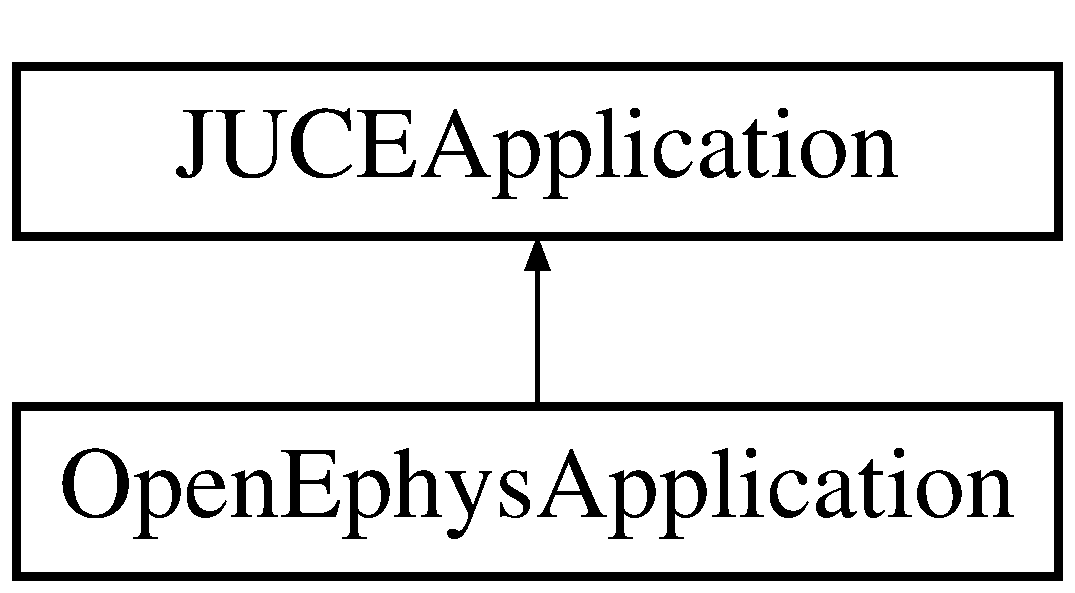
\includegraphics[height=2.000000cm]{class_open_ephys_application}
\end{center}
\end{figure}
\subsection*{Public Member Functions}
\begin{DoxyCompactItemize}
\item 
\mbox{\hyperlink{class_open_ephys_application_a94f33012624a8ec6f5fa3d518027f6fd}{Open\+Ephys\+Application}} ()
\item 
\mbox{\hyperlink{class_open_ephys_application_ac6e352344cd7784bf663b4cc89df69a5}{$\sim$\+Open\+Ephys\+Application}} ()
\item 
void \mbox{\hyperlink{class_open_ephys_application_ab6478b49a9cd18953be1c92b7afd94dc}{initialise}} (const String \&command\+Line)
\item 
void \mbox{\hyperlink{class_open_ephys_application_afc4d64c2d4b6396677a84d5996889e8c}{shutdown}} ()
\item 
void \mbox{\hyperlink{class_open_ephys_application_ab5b3ad9b64ab7d1e4022b967affe3d36}{system\+Requested\+Quit}} ()
\item 
const String \mbox{\hyperlink{class_open_ephys_application_a1ce6b2a2087529f2e26c7031158bfba5}{get\+Application\+Name}} ()
\item 
const String \mbox{\hyperlink{class_open_ephys_application_a44ecd24664080c3d132caaf01cdd6aed}{get\+Application\+Version}} ()
\item 
bool \mbox{\hyperlink{class_open_ephys_application_a6aa18333972da12661f9ee2ea39ed0c5}{more\+Than\+One\+Instance\+Allowed}} ()
\item 
void \mbox{\hyperlink{class_open_ephys_application_af96bfb4d3cb1bf734c75952032de3b70}{another\+Instance\+Started}} (const String \&command\+Line)
\end{DoxyCompactItemize}


\subsection{Detailed Description}
Launches the application and creates the Custom\+Look\+And\+Feel\+Class.

The \mbox{\hyperlink{class_open_ephys_application}{Open\+Ephys\+Application}} class own the application\textquotesingle{}s \mbox{\hyperlink{class_main_window}{Main\+Window}} (via a Scoped\+Pointer).

\begin{DoxySeeAlso}{See also}
\mbox{\hyperlink{class_main_window}{Main\+Window}} 
\end{DoxySeeAlso}


\subsection{Constructor \& Destructor Documentation}
\mbox{\Hypertarget{class_open_ephys_application_a94f33012624a8ec6f5fa3d518027f6fd}\label{class_open_ephys_application_a94f33012624a8ec6f5fa3d518027f6fd}} 
\index{Open\+Ephys\+Application@{Open\+Ephys\+Application}!Open\+Ephys\+Application@{Open\+Ephys\+Application}}
\index{Open\+Ephys\+Application@{Open\+Ephys\+Application}!Open\+Ephys\+Application@{Open\+Ephys\+Application}}
\subsubsection{\texorpdfstring{Open\+Ephys\+Application()}{OpenEphysApplication()}}
{\footnotesize\ttfamily Open\+Ephys\+Application\+::\+Open\+Ephys\+Application (\begin{DoxyParamCaption}{ }\end{DoxyParamCaption})\hspace{0.3cm}{\ttfamily [inline]}}

\mbox{\Hypertarget{class_open_ephys_application_ac6e352344cd7784bf663b4cc89df69a5}\label{class_open_ephys_application_ac6e352344cd7784bf663b4cc89df69a5}} 
\index{Open\+Ephys\+Application@{Open\+Ephys\+Application}!````~Open\+Ephys\+Application@{$\sim$\+Open\+Ephys\+Application}}
\index{````~Open\+Ephys\+Application@{$\sim$\+Open\+Ephys\+Application}!Open\+Ephys\+Application@{Open\+Ephys\+Application}}
\subsubsection{\texorpdfstring{$\sim$\+Open\+Ephys\+Application()}{~OpenEphysApplication()}}
{\footnotesize\ttfamily Open\+Ephys\+Application\+::$\sim$\+Open\+Ephys\+Application (\begin{DoxyParamCaption}{ }\end{DoxyParamCaption})\hspace{0.3cm}{\ttfamily [inline]}}



\subsection{Member Function Documentation}
\mbox{\Hypertarget{class_open_ephys_application_af96bfb4d3cb1bf734c75952032de3b70}\label{class_open_ephys_application_af96bfb4d3cb1bf734c75952032de3b70}} 
\index{Open\+Ephys\+Application@{Open\+Ephys\+Application}!another\+Instance\+Started@{another\+Instance\+Started}}
\index{another\+Instance\+Started@{another\+Instance\+Started}!Open\+Ephys\+Application@{Open\+Ephys\+Application}}
\subsubsection{\texorpdfstring{another\+Instance\+Started()}{anotherInstanceStarted()}}
{\footnotesize\ttfamily void Open\+Ephys\+Application\+::another\+Instance\+Started (\begin{DoxyParamCaption}\item[{const String \&}]{command\+Line }\end{DoxyParamCaption})\hspace{0.3cm}{\ttfamily [inline]}}

\mbox{\Hypertarget{class_open_ephys_application_a1ce6b2a2087529f2e26c7031158bfba5}\label{class_open_ephys_application_a1ce6b2a2087529f2e26c7031158bfba5}} 
\index{Open\+Ephys\+Application@{Open\+Ephys\+Application}!get\+Application\+Name@{get\+Application\+Name}}
\index{get\+Application\+Name@{get\+Application\+Name}!Open\+Ephys\+Application@{Open\+Ephys\+Application}}
\subsubsection{\texorpdfstring{get\+Application\+Name()}{getApplicationName()}}
{\footnotesize\ttfamily const String Open\+Ephys\+Application\+::get\+Application\+Name (\begin{DoxyParamCaption}{ }\end{DoxyParamCaption})\hspace{0.3cm}{\ttfamily [inline]}}

\mbox{\Hypertarget{class_open_ephys_application_a44ecd24664080c3d132caaf01cdd6aed}\label{class_open_ephys_application_a44ecd24664080c3d132caaf01cdd6aed}} 
\index{Open\+Ephys\+Application@{Open\+Ephys\+Application}!get\+Application\+Version@{get\+Application\+Version}}
\index{get\+Application\+Version@{get\+Application\+Version}!Open\+Ephys\+Application@{Open\+Ephys\+Application}}
\subsubsection{\texorpdfstring{get\+Application\+Version()}{getApplicationVersion()}}
{\footnotesize\ttfamily const String Open\+Ephys\+Application\+::get\+Application\+Version (\begin{DoxyParamCaption}{ }\end{DoxyParamCaption})\hspace{0.3cm}{\ttfamily [inline]}}

\mbox{\Hypertarget{class_open_ephys_application_ab6478b49a9cd18953be1c92b7afd94dc}\label{class_open_ephys_application_ab6478b49a9cd18953be1c92b7afd94dc}} 
\index{Open\+Ephys\+Application@{Open\+Ephys\+Application}!initialise@{initialise}}
\index{initialise@{initialise}!Open\+Ephys\+Application@{Open\+Ephys\+Application}}
\subsubsection{\texorpdfstring{initialise()}{initialise()}}
{\footnotesize\ttfamily void Open\+Ephys\+Application\+::initialise (\begin{DoxyParamCaption}\item[{const String \&}]{command\+Line }\end{DoxyParamCaption})\hspace{0.3cm}{\ttfamily [inline]}}

\mbox{\Hypertarget{class_open_ephys_application_a6aa18333972da12661f9ee2ea39ed0c5}\label{class_open_ephys_application_a6aa18333972da12661f9ee2ea39ed0c5}} 
\index{Open\+Ephys\+Application@{Open\+Ephys\+Application}!more\+Than\+One\+Instance\+Allowed@{more\+Than\+One\+Instance\+Allowed}}
\index{more\+Than\+One\+Instance\+Allowed@{more\+Than\+One\+Instance\+Allowed}!Open\+Ephys\+Application@{Open\+Ephys\+Application}}
\subsubsection{\texorpdfstring{more\+Than\+One\+Instance\+Allowed()}{moreThanOneInstanceAllowed()}}
{\footnotesize\ttfamily bool Open\+Ephys\+Application\+::more\+Than\+One\+Instance\+Allowed (\begin{DoxyParamCaption}{ }\end{DoxyParamCaption})\hspace{0.3cm}{\ttfamily [inline]}}

\mbox{\Hypertarget{class_open_ephys_application_afc4d64c2d4b6396677a84d5996889e8c}\label{class_open_ephys_application_afc4d64c2d4b6396677a84d5996889e8c}} 
\index{Open\+Ephys\+Application@{Open\+Ephys\+Application}!shutdown@{shutdown}}
\index{shutdown@{shutdown}!Open\+Ephys\+Application@{Open\+Ephys\+Application}}
\subsubsection{\texorpdfstring{shutdown()}{shutdown()}}
{\footnotesize\ttfamily void Open\+Ephys\+Application\+::shutdown (\begin{DoxyParamCaption}{ }\end{DoxyParamCaption})\hspace{0.3cm}{\ttfamily [inline]}}

\mbox{\Hypertarget{class_open_ephys_application_ab5b3ad9b64ab7d1e4022b967affe3d36}\label{class_open_ephys_application_ab5b3ad9b64ab7d1e4022b967affe3d36}} 
\index{Open\+Ephys\+Application@{Open\+Ephys\+Application}!system\+Requested\+Quit@{system\+Requested\+Quit}}
\index{system\+Requested\+Quit@{system\+Requested\+Quit}!Open\+Ephys\+Application@{Open\+Ephys\+Application}}
\subsubsection{\texorpdfstring{system\+Requested\+Quit()}{systemRequestedQuit()}}
{\footnotesize\ttfamily void Open\+Ephys\+Application\+::system\+Requested\+Quit (\begin{DoxyParamCaption}{ }\end{DoxyParamCaption})\hspace{0.3cm}{\ttfamily [inline]}}



The documentation for this class was generated from the following file\+:\begin{DoxyCompactItemize}
\item 
Source/\mbox{\hyperlink{_main_8cpp}{Main.\+cpp}}\end{DoxyCompactItemize}

\chapter{File Documentation}
\hypertarget{_access_class_8cpp}{}\section{Source/\+Access\+Class.cpp File Reference}
\label{_access_class_8cpp}\index{Source/\+Access\+Class.\+cpp@{Source/\+Access\+Class.\+cpp}}
{\ttfamily \#include \char`\"{}Access\+Class.\+h\char`\"{}}\newline
{\ttfamily \#include \char`\"{}Processors/\+Generic\+Processor/\+Generic\+Processor.\+h\char`\"{}}\newline
{\ttfamily \#include \char`\"{}Processors/\+Message\+Center/\+Message\+Center\+Editor.\+h\char`\"{}}\newline
{\ttfamily \#include \char`\"{}U\+I/\+U\+I\+Component.\+h\char`\"{}}\newline
\subsection*{Namespaces}
\begin{DoxyCompactItemize}
\item 
 \mbox{\hyperlink{namespace_access_class}{Access\+Class}}
\end{DoxyCompactItemize}
\subsection*{Functions}
\begin{DoxyCompactItemize}
\item 
void \mbox{\hyperlink{namespace_access_class_a4f1f8ce54b0d1e3d6319efe95c858e1b}{Access\+Class\+::set\+U\+I\+Component}} (U\+I\+Component $\ast$ui\+\_\+)
\item 
void \mbox{\hyperlink{namespace_access_class_a7a20009ac4b41582f1379b6196f2c07c}{Access\+Class\+::shutdown\+Broadcaster}} ()
\item 
Editor\+Viewport $\ast$ \mbox{\hyperlink{namespace_access_class_a53ff876e8fae76efe1766a3c6b5defc8}{Access\+Class\+::get\+Editor\+Viewport}} ()
\item 
Data\+Viewport $\ast$ \mbox{\hyperlink{namespace_access_class_af26919b327fd17cb4a3ed79623f8795f}{Access\+Class\+::get\+Data\+Viewport}} ()
\item 
Processor\+List $\ast$ \mbox{\hyperlink{namespace_access_class_af8981a34e6624add46145d2a3226c6c7}{Access\+Class\+::get\+Processor\+List}} ()
\item 
Processor\+Graph $\ast$ \mbox{\hyperlink{namespace_access_class_ac50c3de3d49e5d88efb0bdef178523e7}{Access\+Class\+::get\+Processor\+Graph}} ()
\item 
Control\+Panel $\ast$ \mbox{\hyperlink{namespace_access_class_a85b3fce72926c6c93cede477ed7f0dc1}{Access\+Class\+::get\+Control\+Panel}} ()
\item 
Message\+Center\+Editor $\ast$ \mbox{\hyperlink{namespace_access_class_a32785f88b52c58ae0cd1fee7857c1730}{Access\+Class\+::get\+Message\+Center}} ()
\item 
U\+I\+Component $\ast$ \mbox{\hyperlink{namespace_access_class_a847041f47180bab4dd27e7b379f71ce9}{Access\+Class\+::get\+U\+I\+Component}} ()
\item 
Audio\+Component $\ast$ \mbox{\hyperlink{namespace_access_class_a6008b5597fd52fabd69ff28725717287}{Access\+Class\+::get\+Audio\+Component}} ()
\item 
Graph\+Viewer $\ast$ \mbox{\hyperlink{namespace_access_class_a45a325e053c7e866aab251efa1d91008}{Access\+Class\+::get\+Graph\+Viewer}} ()
\item 
Plugin\+Manager $\ast$ \mbox{\hyperlink{namespace_access_class_a23556c0c2fb931081168be89726b7419}{Access\+Class\+::get\+Plugin\+Manager}} ()
\item 
Action\+Broadcaster $\ast$ \mbox{\hyperlink{namespace_access_class_abbdfc97a1cc576d5808d6c9958fdd84f}{Access\+Class\+::get\+Broadcaster}} ()
\end{DoxyCompactItemize}

\hypertarget{_access_class_8h}{}\section{Source/\+Access\+Class.h File Reference}
\label{_access_class_8h}\index{Source/\+Access\+Class.\+h@{Source/\+Access\+Class.\+h}}
{\ttfamily \#include \char`\"{}../\+Juce\+Library\+Code/\+Juce\+Header.\+h\char`\"{}}\newline
\subsection*{Classes}
\begin{DoxyCompactItemize}
\item 
class \mbox{\hyperlink{class_access_class_1_1_external_processor_accessor}{Access\+Class\+::\+External\+Processor\+Accessor}}
\end{DoxyCompactItemize}
\subsection*{Namespaces}
\begin{DoxyCompactItemize}
\item 
 \mbox{\hyperlink{namespace_access_class}{Access\+Class}}
\end{DoxyCompactItemize}
\subsection*{Functions}
\begin{DoxyCompactItemize}
\item 
void \mbox{\hyperlink{namespace_access_class_a4f1f8ce54b0d1e3d6319efe95c858e1b}{Access\+Class\+::set\+U\+I\+Component}} (U\+I\+Component $\ast$ui\+\_\+)
\item 
void \mbox{\hyperlink{namespace_access_class_a7a20009ac4b41582f1379b6196f2c07c}{Access\+Class\+::shutdown\+Broadcaster}} ()
\item 
Editor\+Viewport $\ast$ \mbox{\hyperlink{namespace_access_class_a53ff876e8fae76efe1766a3c6b5defc8}{Access\+Class\+::get\+Editor\+Viewport}} ()
\item 
Data\+Viewport $\ast$ \mbox{\hyperlink{namespace_access_class_af26919b327fd17cb4a3ed79623f8795f}{Access\+Class\+::get\+Data\+Viewport}} ()
\item 
Processor\+List $\ast$ \mbox{\hyperlink{namespace_access_class_af8981a34e6624add46145d2a3226c6c7}{Access\+Class\+::get\+Processor\+List}} ()
\item 
Processor\+Graph $\ast$ \mbox{\hyperlink{namespace_access_class_ac50c3de3d49e5d88efb0bdef178523e7}{Access\+Class\+::get\+Processor\+Graph}} ()
\item 
Control\+Panel $\ast$ \mbox{\hyperlink{namespace_access_class_a85b3fce72926c6c93cede477ed7f0dc1}{Access\+Class\+::get\+Control\+Panel}} ()
\item 
Message\+Center\+Editor $\ast$ \mbox{\hyperlink{namespace_access_class_a32785f88b52c58ae0cd1fee7857c1730}{Access\+Class\+::get\+Message\+Center}} ()
\item 
U\+I\+Component $\ast$ \mbox{\hyperlink{namespace_access_class_a847041f47180bab4dd27e7b379f71ce9}{Access\+Class\+::get\+U\+I\+Component}} ()
\item 
Audio\+Component $\ast$ \mbox{\hyperlink{namespace_access_class_a6008b5597fd52fabd69ff28725717287}{Access\+Class\+::get\+Audio\+Component}} ()
\item 
Graph\+Viewer $\ast$ \mbox{\hyperlink{namespace_access_class_a45a325e053c7e866aab251efa1d91008}{Access\+Class\+::get\+Graph\+Viewer}} ()
\item 
Plugin\+Manager $\ast$ \mbox{\hyperlink{namespace_access_class_a23556c0c2fb931081168be89726b7419}{Access\+Class\+::get\+Plugin\+Manager}} ()
\item 
Action\+Broadcaster $\ast$ \mbox{\hyperlink{namespace_access_class_abbdfc97a1cc576d5808d6c9958fdd84f}{Access\+Class\+::get\+Broadcaster}} ()
\end{DoxyCompactItemize}

\hypertarget{_core_services_8cpp}{}\section{Source/\+Core\+Services.cpp File Reference}
\label{_core_services_8cpp}\index{Source/\+Core\+Services.\+cpp@{Source/\+Core\+Services.\+cpp}}
{\ttfamily \#include \char`\"{}Core\+Services.\+h\char`\"{}}\newline
{\ttfamily \#include \char`\"{}Access\+Class.\+h\char`\"{}}\newline
{\ttfamily \#include \char`\"{}Processors/\+Processor\+Graph/\+Processor\+Graph.\+h\char`\"{}}\newline
{\ttfamily \#include \char`\"{}Processors/\+Record\+Node/\+Record\+Node.\+h\char`\"{}}\newline
{\ttfamily \#include \char`\"{}U\+I/\+Editor\+Viewport.\+h\char`\"{}}\newline
{\ttfamily \#include \char`\"{}U\+I/\+Control\+Panel.\+h\char`\"{}}\newline
{\ttfamily \#include \char`\"{}Processors/\+Message\+Center/\+Message\+Center\+Editor.\+h\char`\"{}}\newline
{\ttfamily \#include \char`\"{}Processors/\+Events/\+Events.\+h\char`\"{}}\newline
\subsection*{Namespaces}
\begin{DoxyCompactItemize}
\item 
 \mbox{\hyperlink{namespace_core_services}{Core\+Services}}
\item 
 \mbox{\hyperlink{namespace_core_services_1_1_record_node}{Core\+Services\+::\+Record\+Node}}
\end{DoxyCompactItemize}
\subsection*{Macros}
\begin{DoxyCompactItemize}
\item 
\#define \mbox{\hyperlink{_core_services_8cpp_a277ebc194fca07cd09e6e6fa2640e27d}{X\+S\+T\+R\+\_\+\+D\+EF}}(s)~\#s
\item 
\#define \mbox{\hyperlink{_core_services_8cpp_a241e54a426d0d7ee02d99ce27dca4cc9}{S\+T\+R\+\_\+\+D\+EF}}(s)~\mbox{\hyperlink{_core_services_8cpp_a277ebc194fca07cd09e6e6fa2640e27d}{X\+S\+T\+R\+\_\+\+D\+EF}}(s)
\end{DoxyCompactItemize}
\subsection*{Functions}
\begin{DoxyCompactItemize}
\item 
void \mbox{\hyperlink{namespace_core_services_a2e53c32783c6caa3d66afb7172dc61fd}{Core\+Services\+::update\+Signal\+Chain}} (Generic\+Editor $\ast$source)
\item 
bool \mbox{\hyperlink{namespace_core_services_a877cdc8ef0b6ea0dce61575de663c6f3}{Core\+Services\+::get\+Recording\+Status}} ()
\item 
void \mbox{\hyperlink{namespace_core_services_a70b56adbc7be044f913f088a162a69fd}{Core\+Services\+::set\+Recording\+Status}} (bool enable)
\item 
bool \mbox{\hyperlink{namespace_core_services_afe3e006d8ad41f122bd0d68b9d5976b0}{Core\+Services\+::get\+Acquisition\+Status}} ()
\item 
void \mbox{\hyperlink{namespace_core_services_a93b4f6a705bead14ce6caa04355b03ba}{Core\+Services\+::set\+Acquisition\+Status}} (bool enable)
\item 
void \mbox{\hyperlink{namespace_core_services_a78fdbd1d2b88cc908e60559b47d8a77e}{Core\+Services\+::send\+Status\+Message}} (const String \&text)
\item 
void \mbox{\hyperlink{namespace_core_services_aafd9eeb68c631f37fa234eee4eb8fbca}{Core\+Services\+::send\+Status\+Message}} (const char $\ast$text)
\item 
void \mbox{\hyperlink{namespace_core_services_a3b017a18a0a09b6c4e2fa4af4c5df11e}{Core\+Services\+::highlight\+Editor}} (Generic\+Editor $\ast$ed)
\item 
juce\+::int64 \mbox{\hyperlink{namespace_core_services_a79defb96087c3bddcb388a29a38d6952}{Core\+Services\+::get\+Global\+Timestamp}} ()
\item 
juce\+::int64 \mbox{\hyperlink{namespace_core_services_ad1083e5525ad9ebd19afd9364f122059}{Core\+Services\+::get\+Software\+Timestamp}} ()
\item 
float \mbox{\hyperlink{namespace_core_services_ac9fb78e241aa3805b05d206c78ecfca1}{Core\+Services\+::get\+Global\+Sample\+Rate}} ()
\item 
float \mbox{\hyperlink{namespace_core_services_a1ce836de202979c7c8a8e4f4d42c87f4}{Core\+Services\+::get\+Software\+Sample\+Rate}} ()
\item 
void \mbox{\hyperlink{namespace_core_services_a5b804cf3cba68340baeb3b7c7173b530}{Core\+Services\+::set\+Recording\+Directory}} (String dir)
\item 
void \mbox{\hyperlink{namespace_core_services_a450d2d9574435570b5e4e38caaeb05d7}{Core\+Services\+::create\+New\+Recording\+Dir}} ()
\item 
void \mbox{\hyperlink{namespace_core_services_a2ea8b92387e1ae7ce51180a3861e528c}{Core\+Services\+::set\+Prepend\+Text\+To\+Recording\+Dir}} (String text)
\item 
void \mbox{\hyperlink{namespace_core_services_a75af2d5d3262b95e16bd51fe28a7e26d}{Core\+Services\+::set\+Append\+Text\+To\+Recording\+Dir}} (String text)
\item 
String \mbox{\hyperlink{namespace_core_services_a03eb76579ab53edf169064232a0e2b62}{Core\+Services\+::get\+Selected\+Record\+Engine\+Id}} ()
\item 
bool \mbox{\hyperlink{namespace_core_services_a5c4ad031dbb70b1ca2824a12e65dec86}{Core\+Services\+::set\+Selected\+Record\+Engine\+Id}} (String id)
\item 
void \mbox{\hyperlink{namespace_core_services_1_1_record_node_a5a5d166b16a7990cda9d1667cca88031}{Core\+Services\+::\+Record\+Node\+::create\+Newrecording\+Dir}} ()
\item 
File \mbox{\hyperlink{namespace_core_services_1_1_record_node_aacbae8c35805cac138be95000a31baa2}{Core\+Services\+::\+Record\+Node\+::get\+Recording\+Path}} ()
\item 
int \mbox{\hyperlink{namespace_core_services_1_1_record_node_a9652eb6869f905f2b131245f62ddaaf1}{Core\+Services\+::\+Record\+Node\+::get\+Recording\+Number}} ()
\item 
int \mbox{\hyperlink{namespace_core_services_1_1_record_node_aae47e9fe985ef57735c937bbe8379fa7}{Core\+Services\+::\+Record\+Node\+::get\+Experiment\+Number}} ()
\item 
void \mbox{\hyperlink{namespace_core_services_1_1_record_node_a9475537f3223762f9e1b852ec8d59811}{Core\+Services\+::\+Record\+Node\+::write\+Spike}} (const Spike\+Event $\ast$spike, const Spike\+Channel $\ast$chan)
\item 
void \mbox{\hyperlink{namespace_core_services_1_1_record_node_a28b8d2f049b63dc524b27a9ae8bc88fe}{Core\+Services\+::\+Record\+Node\+::register\+Spike\+Source}} (Generic\+Processor $\ast$processor)
\item 
int \mbox{\hyperlink{namespace_core_services_1_1_record_node_a78a757804cb37410aeb3349594030895}{Core\+Services\+::\+Record\+Node\+::add\+Spike\+Electrode}} (const Spike\+Channel $\ast$elec)
\item 
const char $\ast$ \mbox{\hyperlink{namespace_core_services_a40705adde6940ed1b94cf880a0cc54a0}{Core\+Services\+::get\+Application\+Resource}} (const char $\ast$name, int \&size)
\item 
File \mbox{\hyperlink{namespace_core_services_a25f9182255aa7c83144c5f65819493bc}{Core\+Services\+::get\+Default\+User\+Save\+Directory}} ()
\item 
String \mbox{\hyperlink{namespace_core_services_a93a10ea82325f2a1baf74ee22e5dbd23}{Core\+Services\+::get\+G\+U\+I\+Version}} ()
\end{DoxyCompactItemize}


\subsection{Macro Definition Documentation}
\mbox{\Hypertarget{_core_services_8cpp_a241e54a426d0d7ee02d99ce27dca4cc9}\label{_core_services_8cpp_a241e54a426d0d7ee02d99ce27dca4cc9}} 
\index{Core\+Services.\+cpp@{Core\+Services.\+cpp}!S\+T\+R\+\_\+\+D\+EF@{S\+T\+R\+\_\+\+D\+EF}}
\index{S\+T\+R\+\_\+\+D\+EF@{S\+T\+R\+\_\+\+D\+EF}!Core\+Services.\+cpp@{Core\+Services.\+cpp}}
\subsubsection{\texorpdfstring{S\+T\+R\+\_\+\+D\+EF}{STR\_DEF}}
{\footnotesize\ttfamily \#define S\+T\+R\+\_\+\+D\+EF(\begin{DoxyParamCaption}\item[{}]{s }\end{DoxyParamCaption})~\mbox{\hyperlink{_core_services_8cpp_a277ebc194fca07cd09e6e6fa2640e27d}{X\+S\+T\+R\+\_\+\+D\+EF}}(s)}

\mbox{\Hypertarget{_core_services_8cpp_a277ebc194fca07cd09e6e6fa2640e27d}\label{_core_services_8cpp_a277ebc194fca07cd09e6e6fa2640e27d}} 
\index{Core\+Services.\+cpp@{Core\+Services.\+cpp}!X\+S\+T\+R\+\_\+\+D\+EF@{X\+S\+T\+R\+\_\+\+D\+EF}}
\index{X\+S\+T\+R\+\_\+\+D\+EF@{X\+S\+T\+R\+\_\+\+D\+EF}!Core\+Services.\+cpp@{Core\+Services.\+cpp}}
\subsubsection{\texorpdfstring{X\+S\+T\+R\+\_\+\+D\+EF}{XSTR\_DEF}}
{\footnotesize\ttfamily \#define X\+S\+T\+R\+\_\+\+D\+EF(\begin{DoxyParamCaption}\item[{}]{s }\end{DoxyParamCaption})~\#s}


\hypertarget{_core_services_8h}{}\section{Source/\+Core\+Services.h File Reference}
\label{_core_services_8h}\index{Source/\+Core\+Services.\+h@{Source/\+Core\+Services.\+h}}
{\ttfamily \#include \char`\"{}../\+Juce\+Library\+Code/\+Juce\+Header.\+h\char`\"{}}\newline
{\ttfamily \#include \char`\"{}Processors/\+Plugin\+Manager/\+Open\+Ephys\+Plugin.\+h\char`\"{}}\newline
\subsection*{Namespaces}
\begin{DoxyCompactItemize}
\item 
 \mbox{\hyperlink{namespace_core_services}{Core\+Services}}
\item 
 \mbox{\hyperlink{namespace_core_services_1_1_record_node}{Core\+Services\+::\+Record\+Node}}
\end{DoxyCompactItemize}
\subsection*{Functions}
\begin{DoxyCompactItemize}
\item 
void \mbox{\hyperlink{namespace_core_services_a2e53c32783c6caa3d66afb7172dc61fd}{Core\+Services\+::update\+Signal\+Chain}} (Generic\+Editor $\ast$source)
\item 
bool \mbox{\hyperlink{namespace_core_services_a877cdc8ef0b6ea0dce61575de663c6f3}{Core\+Services\+::get\+Recording\+Status}} ()
\item 
void \mbox{\hyperlink{namespace_core_services_a70b56adbc7be044f913f088a162a69fd}{Core\+Services\+::set\+Recording\+Status}} (bool enable)
\item 
bool \mbox{\hyperlink{namespace_core_services_afe3e006d8ad41f122bd0d68b9d5976b0}{Core\+Services\+::get\+Acquisition\+Status}} ()
\item 
void \mbox{\hyperlink{namespace_core_services_a93b4f6a705bead14ce6caa04355b03ba}{Core\+Services\+::set\+Acquisition\+Status}} (bool enable)
\item 
void \mbox{\hyperlink{namespace_core_services_a78fdbd1d2b88cc908e60559b47d8a77e}{Core\+Services\+::send\+Status\+Message}} (const String \&text)
\item 
void \mbox{\hyperlink{namespace_core_services_aafd9eeb68c631f37fa234eee4eb8fbca}{Core\+Services\+::send\+Status\+Message}} (const char $\ast$text)
\item 
void \mbox{\hyperlink{namespace_core_services_a3b017a18a0a09b6c4e2fa4af4c5df11e}{Core\+Services\+::highlight\+Editor}} (Generic\+Editor $\ast$ed)
\item 
juce\+::int64 \mbox{\hyperlink{namespace_core_services_a79defb96087c3bddcb388a29a38d6952}{Core\+Services\+::get\+Global\+Timestamp}} ()
\item 
float \mbox{\hyperlink{namespace_core_services_ac9fb78e241aa3805b05d206c78ecfca1}{Core\+Services\+::get\+Global\+Sample\+Rate}} ()
\item 
juce\+::int64 \mbox{\hyperlink{namespace_core_services_ad1083e5525ad9ebd19afd9364f122059}{Core\+Services\+::get\+Software\+Timestamp}} ()
\item 
float \mbox{\hyperlink{namespace_core_services_a1ce836de202979c7c8a8e4f4d42c87f4}{Core\+Services\+::get\+Software\+Sample\+Rate}} ()
\item 
void \mbox{\hyperlink{namespace_core_services_a5b804cf3cba68340baeb3b7c7173b530}{Core\+Services\+::set\+Recording\+Directory}} (String dir)
\item 
void \mbox{\hyperlink{namespace_core_services_a450d2d9574435570b5e4e38caaeb05d7}{Core\+Services\+::create\+New\+Recording\+Dir}} ()
\item 
void \mbox{\hyperlink{namespace_core_services_a2ea8b92387e1ae7ce51180a3861e528c}{Core\+Services\+::set\+Prepend\+Text\+To\+Recording\+Dir}} (String text)
\item 
void \mbox{\hyperlink{namespace_core_services_a75af2d5d3262b95e16bd51fe28a7e26d}{Core\+Services\+::set\+Append\+Text\+To\+Recording\+Dir}} (String text)
\item 
String \mbox{\hyperlink{namespace_core_services_a03eb76579ab53edf169064232a0e2b62}{Core\+Services\+::get\+Selected\+Record\+Engine\+Id}} ()
\item 
bool \mbox{\hyperlink{namespace_core_services_a5c4ad031dbb70b1ca2824a12e65dec86}{Core\+Services\+::set\+Selected\+Record\+Engine\+Id}} (String id)
\item 
void \mbox{\hyperlink{namespace_core_services_1_1_record_node_a5a5d166b16a7990cda9d1667cca88031}{Core\+Services\+::\+Record\+Node\+::create\+Newrecording\+Dir}} ()
\item 
File \mbox{\hyperlink{namespace_core_services_1_1_record_node_aacbae8c35805cac138be95000a31baa2}{Core\+Services\+::\+Record\+Node\+::get\+Recording\+Path}} ()
\item 
int \mbox{\hyperlink{namespace_core_services_1_1_record_node_a9652eb6869f905f2b131245f62ddaaf1}{Core\+Services\+::\+Record\+Node\+::get\+Recording\+Number}} ()
\item 
int \mbox{\hyperlink{namespace_core_services_1_1_record_node_aae47e9fe985ef57735c937bbe8379fa7}{Core\+Services\+::\+Record\+Node\+::get\+Experiment\+Number}} ()
\item 
void \mbox{\hyperlink{namespace_core_services_1_1_record_node_a9475537f3223762f9e1b852ec8d59811}{Core\+Services\+::\+Record\+Node\+::write\+Spike}} (const Spike\+Event $\ast$spike, const Spike\+Channel $\ast$chan)
\item 
void \mbox{\hyperlink{namespace_core_services_1_1_record_node_a28b8d2f049b63dc524b27a9ae8bc88fe}{Core\+Services\+::\+Record\+Node\+::register\+Spike\+Source}} (Generic\+Processor $\ast$processor)
\item 
int \mbox{\hyperlink{namespace_core_services_1_1_record_node_a78a757804cb37410aeb3349594030895}{Core\+Services\+::\+Record\+Node\+::add\+Spike\+Electrode}} (const Spike\+Channel $\ast$elec)
\item 
const char $\ast$ \mbox{\hyperlink{namespace_core_services_a40705adde6940ed1b94cf880a0cc54a0}{Core\+Services\+::get\+Application\+Resource}} (const char $\ast$name, int \&size)
\item 
File \mbox{\hyperlink{namespace_core_services_a25f9182255aa7c83144c5f65819493bc}{Core\+Services\+::get\+Default\+User\+Save\+Directory}} ()
\item 
String \mbox{\hyperlink{namespace_core_services_a93a10ea82325f2a1baf74ee22e5dbd23}{Core\+Services\+::get\+G\+U\+I\+Version}} ()
\end{DoxyCompactItemize}

\hypertarget{_doxygen_main_page_8h}{}\section{Source/\+Doxygen\+Main\+Page.h File Reference}
\label{_doxygen_main_page_8h}\index{Source/\+Doxygen\+Main\+Page.\+h@{Source/\+Doxygen\+Main\+Page.\+h}}

\hypertarget{_main_8cpp}{}\section{Source/\+Main.cpp File Reference}
\label{_main_8cpp}\index{Source/\+Main.\+cpp@{Source/\+Main.\+cpp}}
{\ttfamily \#include \char`\"{}../\+Juce\+Library\+Code/\+Juce\+Header.\+h\char`\"{}}\newline
{\ttfamily \#include \char`\"{}Main\+Window.\+h\char`\"{}}\newline
{\ttfamily \#include \char`\"{}U\+I/\+Look\+And\+Feel/\+Custom\+Look\+And\+Feel.\+h\char`\"{}}\newline
{\ttfamily \#include $<$stdio.\+h$>$}\newline
{\ttfamily \#include $<$fstream$>$}\newline
\subsection*{Classes}
\begin{DoxyCompactItemize}
\item 
class \mbox{\hyperlink{class_open_ephys_application}{Open\+Ephys\+Application}}
\end{DoxyCompactItemize}

\hypertarget{_main_window_8cpp}{}\section{Source/\+Main\+Window.cpp File Reference}
\label{_main_window_8cpp}\index{Source/\+Main\+Window.\+cpp@{Source/\+Main\+Window.\+cpp}}
{\ttfamily \#include \char`\"{}Main\+Window.\+h\char`\"{}}\newline
{\ttfamily \#include \char`\"{}U\+I/\+U\+I\+Component.\+h\char`\"{}}\newline
{\ttfamily \#include \char`\"{}U\+I/\+Editor\+Viewport.\+h\char`\"{}}\newline
{\ttfamily \#include $<$stdio.\+h$>$}\newline

\hypertarget{_main_window_8h}{}\section{Source/\+Main\+Window.h File Reference}
\label{_main_window_8h}\index{Source/\+Main\+Window.\+h@{Source/\+Main\+Window.\+h}}
{\ttfamily \#include \char`\"{}../\+Juce\+Library\+Code/\+Juce\+Header.\+h\char`\"{}}\newline
{\ttfamily \#include \char`\"{}U\+I/\+U\+I\+Component.\+h\char`\"{}}\newline
{\ttfamily \#include \char`\"{}Audio/\+Audio\+Component.\+h\char`\"{}}\newline
{\ttfamily \#include \char`\"{}Processors/\+Processor\+Graph/\+Processor\+Graph.\+h\char`\"{}}\newline
\subsection*{Classes}
\begin{DoxyCompactItemize}
\item 
class \mbox{\hyperlink{class_main_window}{Main\+Window}}
\end{DoxyCompactItemize}

%--- End generated contents ---

% Index
\backmatter
\newpage
\phantomsection
\clearemptydoublepage
\addcontentsline{toc}{chapter}{Index}
\printindex

\end{document}
